\documentclass[11pt]{article}

\usepackage[margin=1in]{geometry}
\usepackage{times}
\usepackage{amsmath,amssymb}
\usepackage{graphicx}
\usepackage{booktabs}
\usepackage{hyperref}
\usepackage{xcolor}
\usepackage{caption}
\usepackage[numbers,sort&compress]{natbib}

\hypersetup{
    colorlinks=true,
    linkcolor=blue,
    citecolor=blue,
    urlcolor=blue
}

\title{\textbf{Full-Corpus Context-Stuffing versus Retrieval-Augmented Generation for Citation-Grounded IoT/OT Threat Verification: A Cost, Latency, and Recall Study}}

\author{Gangadhar Singh Shiva \and Poonam Singh Umakanth}
\date{}

\begin{document}

\maketitle

\begin{abstract}
ClearSight is a citation-grounded threat detection system in which a multimodal large language model classifies rendered IoT/OT network traffic and grounds each classification in a verified CAPEC or CVE citation, checked in real time against a hand-curated reference corpus. Its current design sends the \emph{entire} reference corpus into the prompt on every call (``full-corpus context-stuffing''), which guarantees the correct citation is always available to the model but scales prompt cost linearly with corpus size. This paper investigates the natural alternative, retrieval-augmented generation (RAG), and asks a specific question: under what conditions does retrieval outperform full-corpus context-stuffing, and at what cost to reliability? We build a reproducible experimental harness that (i) characterizes the cost and latency trade-off across a synthetic corpus-size sweep from 100 to 10{,}000 entries, and (ii) measures retrieval recall, with bootstrap 95\% confidence intervals, against a set of 15 real, individually verified CAPEC/CVE entries fetched live from MITRE and NVD, paired with 45 hand-written natural-language queries (three independent paraphrases per entry) designed to avoid trivial lexical overlap with the source text, across three local, fully reproducible retrieval backends (TF-IDF, BM25, and LSA). We find that full-corpus prompt cost grows approximately $100\times$ from 100 to 10{,}000 entries (3{,}485 to 362{,}722 estimated tokens per call) while RAG's prompt cost remains flat regardless of corpus size ($\sim$185--283 tokens per call). Recall@5 on the unpadded 15-entry real corpus is 82--89\% depending on retriever (95\% CI spanning roughly 0.74--0.94) but falls to 67--71\% under synthetic distractor load at 2{,}000 entries and does not exceed 73\% even at $k=20$; the confidence intervals for the three retrievers overlap substantially at every corpus size, indicating the degradation is not an artifact of any single weak method, while the intervals at 15 entries and at 2{,}000 entries do not overlap, indicating the degradation itself is a real effect at this sample size. We argue this shows that the RAG-versus-full-corpus decision is not solely a function of corpus size, as is often assumed, but is gated by retriever quality and corpus composition: a retriever that misses the correct entry converts a reliability guarantee (full-corpus's recall of 1.0 by construction) into a probabilistic one whose failure mode is silent and dangerous in a system whose entire value proposition is trustworthy citation grounding. We release our full experimental harness, including scripts to reconstruct the experiment against the complete public CAPEC catalog and real NVD data with a swappable dense-embedding retriever, to support replication with production-grade retrieval.
\end{abstract}

\section{Introduction}

Grounding large language model outputs in verifiable evidence is increasingly treated as a prerequisite for deploying LLMs in security-critical decision support, where an unverified but plausible-sounding citation can be more dangerous than an obviously fabricated one \citep{clearsight2026}. ClearSight \citep{clearsight2026} is one such system: it renders windows of IoT/OT network traffic as images, classifies them with a multimodal LLM (Claude Sonnet~5), and requires every classification to be accompanied by a citation to a specific CAPEC attack pattern or CVE vulnerability record. Before any alert reaches a human analyst, the cited identifier is checked against a hand-verified local reference corpus built by cross-referencing the official MITRE CAPEC and NIST NVD databases. Reported results for this system on the CIC-IoT-2023 dataset \citep{ciciot2023} show 96.7--100\% classification accuracy across 34 attack types, alongside a critical secondary finding: without a grounding corpus, the model attaches a \emph{real} CAPEC or CVE identifier to the \emph{wrong} explanation in 25--50\% of responses --- a failure mode that is more dangerous than outright fabrication because it is difficult for a human reviewer to catch at a glance.

The grounding mechanism that makes this possible currently works by \emph{context-stuffing}: every classification call places the entire verified reference corpus into the prompt alongside the traffic image, so the model never needs to search for the right entry --- it is always present. The ClearSight authors are explicit that this is a deliberate, disclosed simplification appropriate to a research-stage system with a small corpus, not a claim that it is the right design at scale \citep{clearsight2026}. As the corpus grows with every newly verified CAPEC or CVE entry, every future call becomes larger and more expensive, independent of how many of those entries are actually relevant to a given traffic sample. The obvious alternative is retrieval-augmented generation (RAG) \citep{lewis2020rag}: embed the corpus once, and at inference time retrieve only the top-$k$ entries relevant to the current sample.

This substitution is not free. Full-corpus context-stuffing has an appealing invariant: if the correct entry exists in the corpus, it is always in the prompt, so there is no failure mode in which the correct citation is simply unavailable to the model. RAG trades that invariant for efficiency --- if the retriever ranks the correct entry outside the top-$k$, the model cannot cite it correctly no matter how good the underlying LLM is. For a system whose central claim is that its citations are independently verifiable and trustworthy, this is not a minor implementation detail; it is a question about whether a fundamental safety property survives the transition to a scalable architecture.

\paragraph{Contributions.} This paper makes four contributions:
\begin{enumerate}
    \item We build and release an experimental harness that directly compares full-corpus context-stuffing against RAG retrieval on prompt token cost, estimated dollar cost, and construction latency across a controlled corpus-size sweep from 100 to 10{,}000 entries.
    \item We measure retrieval recall, with bootstrap confidence intervals, against a real, individually verified sub-corpus of 15 CAPEC/CVE entries fetched live from MITRE and NVD (not recalled from memory or templated), paired with 45 hand-written natural-language queries, and show that recall degrades substantially under distractor load and does not fully recover even at large $k$.
    \item We replicate this recall measurement across three independent, fully local retrieval backends (TF-IDF, BM25, LSA) to test whether the degradation is specific to one weak retriever or holds across different classical retrieval methods, and report overlapping confidence intervals across methods alongside non-overlapping intervals across corpus sizes.
    \item We discuss the implication for citation-grounded security systems specifically: that the RAG-versus-full-corpus decision should be conditioned on measured retriever recall, not on corpus size alone, and we release a reproducible pipeline (including bulk CAPEC/NVD fetchers and a pluggable dense-embedding interface) for re-running this study with production-grade retrieval.
\end{enumerate}

\section{Related Work}

\textbf{Retrieval-augmented generation.} \citet{lewis2020rag} introduced RAG as a general architecture for combining a parametric language model with a non-parametric retrieval index, motivated primarily by knowledge-intensive NLP tasks where the full knowledge source cannot fit in context. Our setting differs in scale and in stakes: ClearSight's reference corpus is currently small enough to fit in context entirely, and the question is not whether retrieval is \emph{necessary} but whether it is \emph{safe} to adopt for a system whose grounding guarantee is part of its trust model.

\textbf{Classical retrieval methods.} We evaluate three retrieval backends spanning several decades of information retrieval research. TF-IDF with cosine similarity is a standard sparse vector-space baseline. Okapi BM25 \citep{robertson2009bm25} refines term-frequency scoring with saturation and document-length normalization and remains the default lexical baseline against which most modern dense retrievers are compared. Latent Semantic Analysis \citep{deerwester1990lsa} projects TF-IDF vectors into a lower-dimensional space via truncated singular value decomposition, capturing co-occurrence structure that exact-vocabulary matching methods miss, without requiring an external neural embedding model. We use these three specifically because they are the strongest retrieval methods available without downloading external model weights, which was infeasible in the network-restricted environment this study was conducted in (Section~\ref{sec:limitations}).

\textbf{Hallucination and grounding in security-domain LLMs.} Survey evidence cited in the ClearSight report indicates both rapid adoption and rising concern: a May 2026 ISC2 survey of 856 security professionals found widespread worry about AI fabrication and demand for verifiable AI decisions, and a 2026 SANS survey found 78\% of security teams actively using generative AI daily while 63\% report it falls short in real detection and response work \citep{clearsight2026}. This gap between adoption and verifiability is the direct motivation for citation-grounded architectures such as ClearSight, and by extension for understanding the reliability properties of any retrieval layer placed inside such a system.

\textbf{IoT/OT threat detection.} CIC-IoT-2023 \citep{ciciot2023} is a labeled dataset of real IoT botnet traffic spanning 33 attack types across 7 categories plus benign traffic, collected from 105 real IoT devices. It is the traffic dataset underlying ClearSight's classification evaluation and, indirectly, the attack taxonomy that motivates the CAPEC/CVE entries used as retrieval targets in this study.

\section{Methodology}

\subsection{Two context-construction strategies}

We implement both strategies behind a common interface so they can be compared under identical query sets and identical corpora.

\textbf{Full-corpus context-stuffing.} Every classification call serializes every entry in the reference corpus into the prompt, concatenated with the query. Retrieval recall is 1.0 by construction: if the correct entry exists anywhere in the corpus, it is present in every call.

\textbf{RAG retrieval.} An index is built once per corpus (an amortized, one-time cost). At query time, the top-$k$ most similar entries are retrieved and only those are placed in the prompt. We evaluate three interchangeable retrieval backends behind a common \texttt{fit()}/\texttt{similarities()} interface: TF-IDF with cosine similarity (scikit-learn's \texttt{TfidfVectorizer} \citep{scikit-learn}), Okapi BM25 \citep{robertson2009bm25} (via the \texttt{rank\_bm25} package), and LSA (TF-IDF followed by truncated SVD \citep{deerwester1990lsa}, via scikit-learn's \texttt{TruncatedSVD}). All three run fully locally with no external model download. The same interface additionally supports a dense sentence-embedding model (\texttt{sentence-transformers}) as a drop-in fourth backend; we were unable to execute this configuration in this study for reasons detailed in Section~\ref{sec:limitations}, and report it as the clearest direction for follow-up work.

\subsection{Cost and latency measurement}

Prompt token counts are estimated with a fixed heuristic of 1.3 tokens per whitespace-delimited word, a standard approximation for English technical text under byte-pair-encoding tokenizers. This is not an exact count from a production tokenizer, but the approximation is applied identically to both strategies, so the \emph{relative} comparison it produces --- the primary quantity of interest --- is meaningful even where the absolute token counts are offset by a constant factor. Dollar costs are derived from this token estimate using a placeholder per-million-token input price; because pricing changes over time and by model tier, we report token counts as the primary cost metric and treat dollar figures as illustrative. Latency is measured as wall-clock time to construct the context for a single query (string concatenation for full-corpus; similarity search and result assembly for RAG), using \texttt{time.perf\_counter()}; this measures context-construction overhead only, not end-to-end LLM inference latency, which is dominated by the model call itself and is outside the scope of this study.

\subsection{Corpus construction}

We use two corpora for two different purposes.

\textbf{Synthetic corpus-size sweep (cost/latency characterization).} To characterize how cost and latency scale with corpus size independent of any particular corpus's content, we construct synthetic corpora at sizes $\{100, 500, 1{,}000, 2{,}000, 5{,}000, 10{,}000\}$. Each corpus contains 20 fixed anchor entries modeled on real CAPEC/CVE structure (including CAPEC-482 TCP Flood, CAPEC-488 HTTP Flood, and CVE-2016-10401, drawn directly from the ClearSight report's published examples), padded with deterministically seeded synthetic distractor entries generated from a template vocabulary of protocols, attack families, and severity language, to reach the target size. This construction isolates the scaling behavior of the two strategies, which is a property of prompt construction, not of corpus semantics.

\textbf{Real corpus (recall evaluation).} Because the quantity we most care about --- whether the correct citation is actually retrievable --- \emph{is} data-dependent, we do not rely on the synthetic corpus for our recall claims. We instead fetched 15 real CAPEC and CVE entries individually and live from \url{capec.mitre.org} and \url{nvd.nist.gov} during this study (12 CAPEC attack patterns and 3 CVE records relevant to IoT botnet compromise, listed in Table~\ref{tab:real-entries}), transcribing each entry's actual name, description, and source citation rather than relying on recalled or templated text. This verification process itself surfaced two errors in an earlier, unverified draft of the corpus: CAPEC-98 was assumed to describe port scanning but is actually \emph{Phishing} (the correct identifier for port scanning is CAPEC-300), and CAPEC-153 was assumed to describe command injection but is actually \emph{Input Data Manipulation}. Both were corrected before the experiments reported here. We consider this an informative anecdote rather than a footnote: it is a small, unplanned demonstration of exactly the citation-mismatch failure mode that motivates ClearSight's verification layer in the first place.

For each real anchor entry we hand-wrote three independent natural-language queries describing plausible observed traffic behavior (45 queries total), written independently of the entry's own description text and independently of each other, to avoid trivially inflating lexical retrieval performance through shared vocabulary and to reduce the granularity of the resulting recall estimate. For example, the three queries for CAPEC-482 (TCP Flood) describe, respectively, ``sustained high-rate SYN packets with no completed handshake,'' ``a firewall log [showing] thousands of half-open connection attempts per second from a single source,'' and ``server resource exhaustion coincid[ing] with a spike in connection-state table entries, no data exchanged'' --- three different observational framings of the same underlying attack, none of which closely mirrors the entry's own formal description. With 15 queries, a single query flipping between hit and miss moves the recall estimate by 6.7 percentage points; with 45, by 2.2 points, which is the primary reason we expanded the query set beyond our initial 15-query pilot. To study recall under distractor load, corpus sizes beyond the 15 real anchors ($\{15, 50, 100, 500, 1{,}000, 2{,}000\}$) are padded with the same synthetic distractor generator used in the cost/latency sweep. We are explicit that this makes the \emph{background noise} synthetic while the \emph{anchors and queries} --- the entities recall is measured against --- are entirely real; Section~\ref{sec:limitations} discusses what a fully real corpus at this scale would require.

\begin{table}[t]
\centering
\caption{Real CAPEC/CVE anchor entries, individually fetched and verified.}
\label{tab:real-entries}
\small
\begin{tabular}{ll}
\toprule
Identifier & Name \\
\midrule
CAPEC-482 & TCP Flood \\
CAPEC-488 & HTTP Flood \\
CAPEC-486 & UDP Flood \\
CAPEC-487 & ICMP Flood \\
CAPEC-300 & Port Scanning \\
CAPEC-49 & Password Brute Forcing \\
CAPEC-94 & Adversary in the Middle (AiTM) \\
CAPEC-141 & Cache Poisoning \\
CAPEC-66 & SQL Injection \\
CAPEC-63 & Cross-Site Scripting (XSS) \\
CAPEC-137 & Parameter Injection \\
CAPEC-153 & Input Data Manipulation \\
CVE-2016-10401 & ZyXEL PK5001Z default \texttt{su} password \\
CVE-2017-17215 & Huawei HG532 remote code execution \\
CVE-2014-9583 & ASUS WRT \texttt{infosvr} command execution backdoor \\
\bottomrule
\end{tabular}
\end{table}

\subsection{Experimental protocol}

All experiments use a fixed random seed (42) for corpus construction so results are exactly reproducible. Each condition (strategy $\times$ retriever $\times$ corpus size $\times$ $k$) is evaluated over the full query set repeated 2--3 times to smooth latency measurement noise (90--180 total query evaluations per condition on the 45-query real set); recall is deterministic given the seed and is unaffected by repetition. We report mean token count, mean estimated cost, mean latency, one-time index build time, and recall@$k$ (whether the ground-truth entry ID appears among what is placed in the prompt).

For every recall estimate on the real query set we additionally compute a 95\% confidence interval via nonparametric bootstrap: we resample the 45 (or 90, with repeats) binary hit/miss outcomes with replacement 10{,}000 times, compute the mean recall of each resample, and report the 2.5th and 97.5th percentiles of the resulting distribution. This lets us distinguish a genuine difference in recall (non-overlapping intervals) from noise at this sample size (overlapping intervals), rather than presenting bare point estimates as in an earlier 15-query pilot version of this experiment.

\section{Results}

\subsection{Cost and latency scale as predicted by architecture, not by corpus content}

Table~\ref{tab:synthetic-cost} shows prompt token cost as a function of corpus size for both strategies. Full-corpus token cost grows linearly with corpus size, from an estimated 3{,}485 tokens per call at 100 entries to 362{,}722 tokens per call at 10{,}000 entries --- approximately a $104\times$ increase for a $100\times$ increase in corpus size, consistent with the expected linear relationship. RAG's token cost remains essentially flat across the same range (185--194 tokens per call at $k=5$), because it only ever places $k$ entries in the prompt regardless of how large the underlying corpus is. Index build time for RAG (TF-IDF fitting) grows from 3~ms at 100 entries to 84~ms at 10{,}000 entries, a one-time cost per corpus update rather than a per-call cost. Figure~\ref{fig:cost} visualizes this trade-off.

\begin{table}[t]
\centering
\caption{Prompt token cost vs.\ corpus size, synthetic sweep, $k=5$ for RAG.}
\label{tab:synthetic-cost}
\small
\begin{tabular}{rrrrr}
\toprule
Corpus size & Full-corpus tokens & RAG tokens & Full-corpus \$/call & RAG \$/call \\
\midrule
100 & 3{,}485 & 188 & 0.0105 & 0.0006 \\
500 & 18{,}375 & 181 & 0.0551 & 0.0005 \\
1{,}000 & 36{,}456 & 186 & 0.1094 & 0.0006 \\
2{,}000 & 72{,}635 & 194 & 0.2179 & 0.0006 \\
5{,}000 & 181{,}718 & 189 & 0.5452 & 0.0006 \\
10{,}000 & 362{,}722 & 185 & 1.0882 & 0.0006 \\
\bottomrule
\end{tabular}
\end{table}

\begin{figure}[t]
\centering
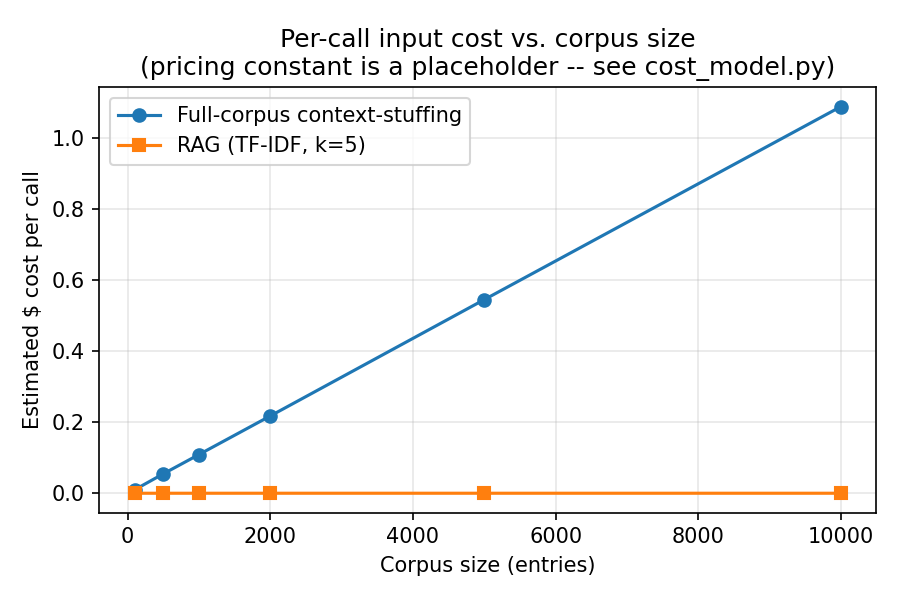
\includegraphics[width=0.75\linewidth]{fig2_cost_vs_corpus_size.png}
\caption{Estimated per-call input cost vs.\ corpus size. Full-corpus cost scales linearly with corpus size; RAG cost is flat. Dollar figures use a placeholder per-token price (Section~3.2) and should be read as illustrating the scaling relationship rather than as a final cost estimate.}
\label{fig:cost}
\end{figure}

\subsection{Retrieval recall degrades under distractor load, consistently across three retrievers, and does not fully recover with larger $k$}

On the unpadded, 15-entry real corpus --- no synthetic distractors --- recall@5 ranges from 82.2\% (BM25) to 88.9\% (TF-IDF and LSA), with bootstrap 95\% confidence intervals of roughly [0.74, 0.94] for all three, confirming all three retrieval mechanisms function correctly on real text and that the small differences between them are not distinguishable at this sample size. As synthetic distractor volume is added, recall falls for all three methods together: by 500 entries, TF-IDF, BM25, and LSA recall have converged to 66.7--68.9\%, and they remain in that band through 2{,}000 entries (Table~\ref{tab:strong-recall}, Figure~\ref{fig:strong-recall-size}). Full-corpus recall is 1.0 at every corpus size, by construction, and its interval (a point mass, by construction of the strategy) never overlaps any RAG configuration's interval past 15 entries.

Two comparisons matter here. First, \emph{across retrievers at a fixed corpus size}, confidence intervals overlap substantially at every size we tested --- e.g. at 2{,}000 entries, TF-IDF is 0.711 [0.622, 0.800], BM25 is 0.667 [0.567, 0.767], and LSA is 0.689 [0.589, 0.778] --- so this study cannot claim any one of these three classical methods is reliably better than another. Second, \emph{across corpus sizes for a fixed retriever}, the intervals do not overlap: TF-IDF at 15 entries is [0.822, 0.944] and at 2{,}000 entries is [0.622, 0.800], a gap of roughly ten points between interval edges. Taken together, this is evidence that the degradation itself is a real, sample-size-robust effect, while the specific choice among these three sparse/lexical-adjacent methods is not what drives it --- consistent with our discussion-section hypothesis that the effect is about the general limits of non-dense retrieval on paraphrased queries, not an artifact of one particular weak implementation.

\begin{table}[t]
\centering
\caption{Recall@5 (95\% bootstrap CI) vs.\ corpus size, real 15-entry anchor set with 45 queries (padded with synthetic distractors beyond 15 entries).}
\label{tab:strong-recall}
\small
\begin{tabular}{rrrrr}
\toprule
Corpus size & Full-corpus & TF-IDF & BM25 & LSA \\
\midrule
15 (real only) & 1.000 & 0.889 [.822, .944] & 0.822 [.744, .900] & 0.889 [.822, .944] \\
50 & 1.000 & 0.867 [.789, .933] & 0.733 [.633, .822] & 0.844 [.767, .911] \\
100 & 1.000 & 0.822 [.744, .900] & 0.711 [.611, .800] & 0.822 [.744, .900] \\
500 & 1.000 & 0.689 [.589, .778] & 0.689 [.589, .778] & 0.667 [.567, .767] \\
1{,}000 & 1.000 & 0.689 [.589, .778] & 0.667 [.567, .767] & 0.667 [.567, .767] \\
2{,}000 & 1.000 & 0.711 [.622, .800] & 0.667 [.567, .767] & 0.689 [.589, .778] \\
\bottomrule
\end{tabular}
\end{table}

\begin{figure}[t]
\centering
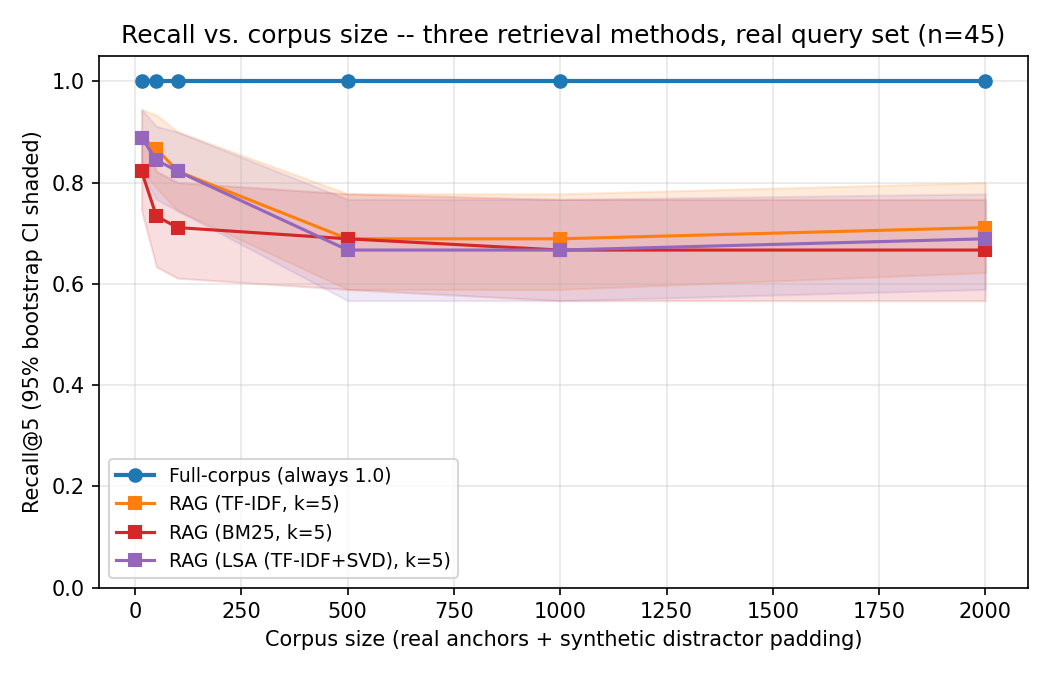
\includegraphics[width=0.85\linewidth]{fig10_strong_recall_vs_corpus_size.png}
\caption{Recall@5 vs.\ corpus size, three retrieval methods, real 45-query set, 95\% bootstrap CI shaded. Full-corpus recall is 1.0 by construction. All three RAG methods degrade together and their intervals overlap at every corpus size.}
\label{fig:strong-recall-size}
\end{figure}

We further ask whether retrieving more candidates ($k$) compensates for this degradation at the largest tested corpus size (2{,}000 entries). Table~\ref{tab:strong-recall-k} and Figure~\ref{fig:strong-recall-k} show that for all three retrievers, increasing $k$ from 1 to 20 raises recall substantially off its floor (roughly 0.42--0.49 at $k=1$) but plateaus in the low-to-mid 70s by $k=15$--20, well short of full-corpus's guaranteed 1.0. The marginal gain from $k=5$ to $k=20$ is small (2--4 percentage points for all three methods) relative to the $\sim$3$\times$ increase in prompt tokens this requires. BM25's per-query latency (roughly 2.0~ms) is markedly higher than TF-IDF's or LSA's (0.36--0.45~ms) in our implementation, reflecting Python-level per-token scoring in the \texttt{rank\_bm25} library rather than a fundamental property of BM25 itself; a production BM25 implementation (e.g., Lucene/Elasticsearch) would not be expected to carry this overhead.

\begin{table}[t]
\centering
\caption{Recall@$k$ (95\% bootstrap CI), real 45-query set, corpus size 2{,}000, three retrievers.}
\label{tab:strong-recall-k}
\small
\begin{tabular}{rrrr}
\toprule
$k$ & TF-IDF & BM25 & LSA \\
\midrule
1 & 0.489 [.389, .589] & 0.422 [.322, .522] & 0.467 [.367, .567] \\
3 & 0.667 [.567, .756] & 0.644 [.544, .744] & 0.644 [.544, .744] \\
5 & 0.711 [.622, .800] & 0.667 [.567, .767] & 0.689 [.589, .778] \\
10 & 0.711 [.622, .800] & 0.689 [.589, .778] & 0.689 [.589, .778] \\
15 & 0.733 [.644, .822] & 0.711 [.611, .800] & 0.711 [.622, .800] \\
20 & 0.733 [.644, .822] & 0.711 [.611, .800] & 0.711 [.622, .800] \\
\bottomrule
\end{tabular}
\end{table}

\begin{figure}[t]
\centering
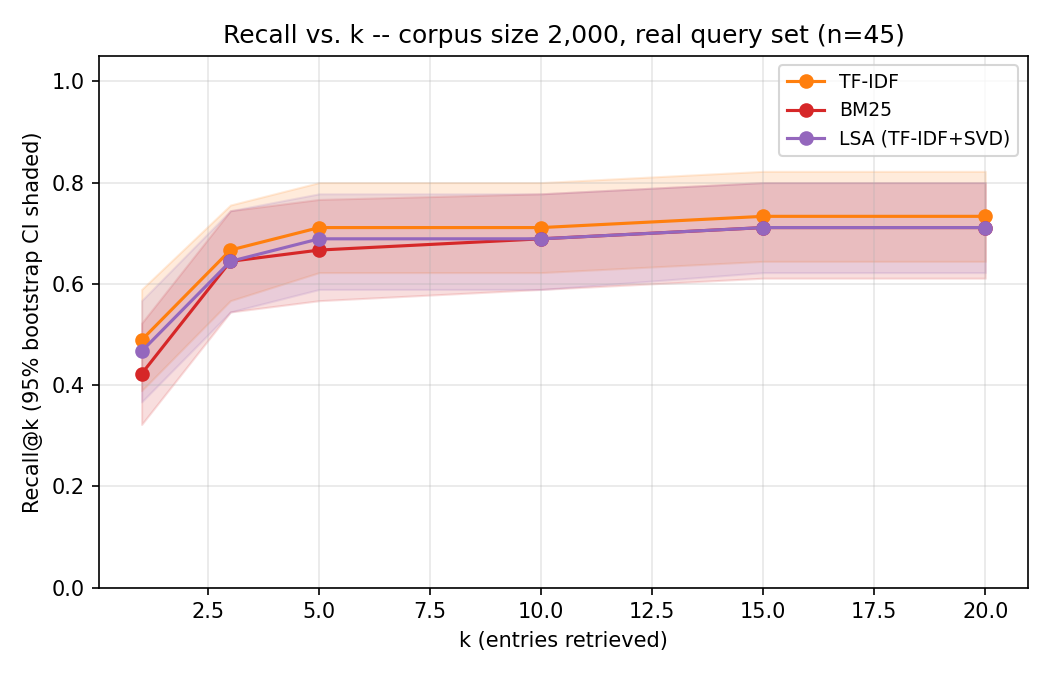
\includegraphics[width=0.85\linewidth]{fig11_strong_recall_vs_k.png}
\caption{Recall vs.\ $k$ at corpus size 2{,}000, three retrieval methods, real 45-query set, 95\% bootstrap CI shaded. All three plateau well below full-corpus's guaranteed recall of 1.0.}
\label{fig:strong-recall-k}
\end{figure}

\section{Discussion}

The two results in this study point in different directions and, taken together, argue against treating ``switch to RAG once the corpus is large'' as a context-independent rule.

The cost and latency result (Section 4.1) is close to a pure consequence of architecture: concatenating $k$ fixed entries per call versus concatenating all $n$ entries per call will produce a flat-versus-linear cost curve for essentially any corpus, real or synthetic, because it follows from how many tokens are placed in the prompt rather than from what those tokens say. We expect this part of our finding to transfer directly to ClearSight's actual production corpus.

The recall result (Section 4.2) is not architecture-level in the same way --- it is a property of how well a retriever ranks a corpus against queries, and it could in principle have been a property of one particular weak implementation rather than a general phenomenon. This is precisely why we replicated the measurement across three independent retrieval methods (TF-IDF, BM25, LSA) instead of reporting a single retriever's numbers: all three degrade together, and their confidence intervals overlap at every corpus size we tested, while the interval at 15 entries and the interval at 2{,}000 entries do not overlap for any of the three. That pattern is what lets us argue the degradation is a real effect of corpus growth under lexical competition, not an artifact of TF-IDF specifically --- three different vector-space and probabilistic ranking methods, including one (LSA) that explicitly captures latent co-occurrence structure beyond exact vocabulary matching, all land in the same 66--71\% band at 2{,}000 entries.

That said, all three methods we tested are still \emph{sparse or sparse-derived}: they operate on term statistics (TF-IDF, BM25) or a linear projection of term statistics (LSA), rather than on a learned semantic embedding space. Our query set was deliberately constructed so that queries describe \emph{observed traffic behavior} in language that does not closely mirror the \emph{formal attack-pattern description} in the corpus entry (Section 3.3) --- a realistic stress test, since an analyst's or a vision model's natural-language description of what traffic looks like will rarely echo a CAPEC entry's formal prose --- and this is precisely the case dense embedding models are designed to handle better, since they match on learned semantic similarity rather than surface or latent-linear term co-occurrence. We therefore expect, but did not measure, meaningfully higher recall from a dense embedding retriever on the same query set; Section~\ref{sec:limitations} details why this comparison could not be completed within this study and how to reproduce it. Until it is, the honest summary of Section 4.2 is narrower than ``RAG is unsafe here'': it is that three different classical retrieval methods, spanning exact and latent lexical matching, all fail to preserve full-corpus's recall guarantee on this query set, which shifts the burden of proof onto whichever retriever a production deployment actually chooses, rather than settling the question in RAG's favor by default.

The practical implication for a system like ClearSight is that the decision to move from full-corpus context-stuffing to RAG should not be gated on corpus size alone, contrary to the framing in the original design document, which treats retrieval as primarily a ``when we scale up'' problem \citep{clearsight2026}. Full-corpus's recall of 1.0 is not merely convenient; it is the property that lets ClearSight's citation-verification layer make the strong claim that grounding failures come only from the language model's own citation behavior, never from missing evidence. Adopting RAG converts this into a probabilistic guarantee whose failure mode --- the correct citation silently absent from the context the model ever sees --- is invisible at the point of failure and can only be detected by exactly the kind of offline recall measurement performed in this paper. We suggest that any production adoption of RAG in this system should be conditioned on a measured recall\@$k$ above an explicit threshold (chosen to keep the system's overall reliability guarantee intact) on the corpus and query distribution actually in use, re-measured whenever the corpus or retriever changes, rather than adopted as a default once a corpus-size threshold is crossed.

\section{Limitations}
\label{sec:limitations}

We are explicit about what this study does and does not establish, both because the underlying system is safety-relevant and because we release the harness for others to extend.

\textbf{No dense embedding model was evaluated.} All recall results use TF-IDF, BM25, or LSA --- three real, established, but sparse or sparse-derived retrieval methods. We built a pluggable embedding interface intended to support a local \texttt{sentence-transformers} model (e.g., \texttt{all-MiniLM-L6-v2}) as a fourth, drop-in backend, and attempted three independent routes to a working dense embedding model within this study: installing \texttt{sentence-transformers} and \texttt{fastembed} (both installed successfully as Python packages but require downloading model weights from \url{huggingface.co} at first use), and installing a spaCy model directly from a GitHub release asset. All three were blocked at the network layer: the sandboxed environment returned HTTP 403 (``blocked-by-allowlist'') for \url{huggingface.co}, for \url{raw.githubusercontent.com}, and for GitHub's release-asset CDN (\url{release-assets.githubusercontent.com}), while \texttt{pip install} against PyPI and page-at-a-time fetches of individual CAPEC/NVD pages remained available throughout. We report this not to relitigate the point but so that a reader attempting to reproduce this study elsewhere knows exactly which network paths must be open. Our recall numbers should be read as a plausible \emph{lower bound} on what a production dense-embedding retriever would achieve on the same queries, not as representative of RAG's ceiling; Section 5 argues that the consistency of the degradation across three sparse/sparse-derived methods is nonetheless informative on its own terms.

\textbf{The corpus used for recall evaluation is not the full public CAPEC/NVD corpus.} We individually fetched and verified 15 real entries rather than performing a bulk download, because the same network environment blocked bulk XML/CSV downloads from \texttt{capec.mitre.org} and direct API access to \texttt{services.nvd.nist.gov} at the sandbox proxy layer; a page-at-a-time fetch tool remained available and was used to obtain the 15 entries reported here, but does not scale to the full $\sim$559-pattern CAPEC catalog or a broad CVE sample within a single research session. We provide bulk-fetch scripts (\texttt{fetch\_capec\_bulk.py}, \texttt{fetch\_nvd\_bulk.py}) that are confirmed to construct and parse requests correctly (verified against a hand-constructed sample) and are expected to succeed on a machine without this network restriction, along with a corpus-merging script and an experiment runner parameterized to use the resulting corpus directly, with no synthetic padding required.

\textbf{Corpus padding beyond 15 entries is synthetic.} The anchors and queries that recall is measured against are entirely real; the distractor entries used to reach larger corpus sizes are synthetically generated. We view this as a reasonable way to study degradation under increasing candidate volume without waiting on a bulk real-data fetch, but it means the absolute recall values at 500--2{,}000 entries reflect a mix of real and synthetic corpus content, and could differ somewhat from recall on an equally sized fully real corpus with different vocabulary statistics.

\textbf{The query set, though expanded, is still modest, and its three paraphrases per anchor are not fully independent.} Forty-five queries is an improvement over an initial 15-query pilot but is still small by information-retrieval evaluation standards, and our bootstrap procedure treats all 45 (or 90, with repeats) hit/miss outcomes as exchangeable, when in fact three queries per anchor entry share an underlying ``topic'' and are likely to succeed or fail together more often than three queries drawn independently across topics would. This means our reported confidence intervals are probably somewhat narrower than the true sampling uncertainty over the space of possible queries an analyst or vision model might produce; a cluster-aware or per-anchor-block bootstrap would be a more conservative and more correct choice for a camera-ready version of this study.

\textbf{Token counts are estimated, not measured from a production tokenizer.} We use a fixed 1.3-tokens-per-word heuristic (Section 3.2). Because the same heuristic applies to both strategies, we expect the qualitative cost-scaling comparison to be robust to this approximation, but absolute dollar figures should not be cited without confirming current model pricing.

\textbf{This study measures retrieval, not end-to-end classification accuracy.} We measure whether the correct citation is \emph{available} to the model, which is necessary but not sufficient for the model to \emph{use} it correctly --- ClearSight's own reported 25--50\% wrong-explanation rate shows that citation availability does not guarantee citation correctness. No multimodal classification calls were made in this study; connecting retrieval recall to downstream classification and citation accuracy requires the live model integration point noted in our release (\texttt{strategies.py}) and is left to future work.

\section{Future Work}

The most direct extension is completing this study with unrestricted network access: running \texttt{run\_all.sh} to fetch the full public CAPEC catalog and a broader real CVE sample, and rerunning the recall sweep with a dense embedding retriever, to obtain a fully real, production-representative recall estimate rather than the bound reported here. A second extension connects this retrieval-layer study to ClearSight's end-to-end metrics by wiring retrieved context into live multimodal classification calls and re-measuring the wrong-explanation and appropriate-abstention rates under RAG versus full-corpus conditions, which would test our discussion-section hypothesis directly rather than by inference from recall alone. A third extension would characterize recall as a function of corpus \emph{semantic density} (how many near-duplicate or closely related entries exist) rather than raw size, since our distractor generator was designed to create genuine lexical competition and a real, larger CAPEC/CVE corpus may or may not exhibit the same density.

\section{Conclusion}

We compared full-corpus context-stuffing against RAG retrieval for ClearSight's citation-grounding layer along the two axes that matter for a production decision: cost/latency and reliability. Cost and latency favor RAG by a wide and predictable margin regardless of corpus content, scaling flat instead of linearly with corpus size. Reliability, measured as retrieval recall with bootstrap confidence intervals against a real, verified CAPEC/CVE query set across three independent retrieval methods, does not transfer for free: TF-IDF, BM25, and LSA all lose 20--30 percentage points of recall under realistic distractor load, converge to overlapping confidence intervals with each other at every corpus size tested, and do not recover with a larger retrieval budget even at $k=20$. That three different classical retrieval methods degrade together, rather than one weak method degrading alone, is evidence that this is a property of sparse and sparse-derived retrieval on paraphrased security queries generally, not an artifact of a single poor implementation --- though whether a dense embedding model closes this gap remains an open, and in our view likely, possibility that this study could not test. We conclude that the choice between full-corpus and RAG designs should be treated as a measured, retriever-specific reliability question with an explicit recall threshold, rather than a corpus-size threshold, and we release our experimental harness, including a fully real-data pipeline and a pluggable dense-embedding interface, to support that measurement as ClearSight's corpus grows.

\section*{Reproducibility}

All code, the real (verified) corpus entries, the synthetic corpus generator, experiment scripts, and plotting scripts used in this paper are released alongside it. The synthetic and real-anchor experiments reported in Sections 4.1--4.2 run without network access and reproduce exactly given the fixed seed (42). The full-real-data extension described in Section~\ref{sec:limitations} requires unrestricted outbound network access and is provided as \texttt{run\_all.sh}.

\bibliographystyle{plainnat}
\begin{thebibliography}{9}

\bibitem[Bhaskaran et al.(2026)]{clearsight2026}
Bhaskaran, A., Ponnavaikko, P., and Shiva, G.~S. (2026).
\newblock ClearSight Multimodal Network Security: Citation-Grounded, Hallucination-Reduced IoT/OT Threat Detection.
\newblock \emph{Problem Framing Report}, Extreme Networks.

\bibitem[Lewis et al.(2020)]{lewis2020rag}
Lewis, P., Perez, E., Piktus, A., Petroni, F., Karpukhin, V., Goyal, N., K\"uttler, H., Lewis, M., Yih, W., Rockt\"aschel, T., Riedel, S., and Kiela, D. (2020).
\newblock Retrieval-Augmented Generation for Knowledge-Intensive NLP Tasks.
\newblock In \emph{Advances in Neural Information Processing Systems 33 (NeurIPS 2020)}.

\bibitem[Robertson and Zaragoza(2009)]{robertson2009bm25}
Robertson, S. and Zaragoza, H. (2009).
\newblock The Probabilistic Relevance Framework: BM25 and Beyond.
\newblock \emph{Foundations and Trends in Information Retrieval}, 3(4), 333--389.

\bibitem[Deerwester et al.(1990)]{deerwester1990lsa}
Deerwester, S., Dumais, S.T., Furnas, G.W., Landauer, T.K., and Harshman, R. (1990).
\newblock Indexing by Latent Semantic Analysis.
\newblock \emph{Journal of the American Society for Information Science}, 41(6), 391--407.

\bibitem[Neto et al.(2023)]{ciciot2023}
Neto, E.C.P., Dadkhah, S., Ferreira, R., Zohourian, A., Lu, R., and Ghorbani, A.A. (2023).
\newblock CICIoT2023: A Real-Time Dataset and Benchmark for Large-Scale Attacks in IoT Environment.
\newblock \emph{Sensors}, 23(13), 5941. \url{https://doi.org/10.3390/s23135941}

\bibitem[Pedregosa et al.(2011)]{scikit-learn}
Pedregosa, F., Varoquaux, G., Gramfort, A., Michel, V., Thirion, B., Grisel, O., Blondel, M., Prettenhofer, P., Weiss, R., Dubourg, V., Vanderplas, J., Passos, A., Cournapeau, D., Brucher, M., Perrot, M., and Duchesnay, E. (2011).
\newblock Scikit-learn: Machine Learning in Python.
\newblock \emph{Journal of Machine Learning Research}, 12, 2825--2830.

\bibitem[MITRE(2026)]{capec}
MITRE Corporation.
\newblock Common Attack Pattern Enumeration and Classification (CAPEC), Version 3.9.
\newblock \url{https://capec.mitre.org}, accessed 2026.

\bibitem[NIST(2026)]{nvd}
National Institute of Standards and Technology.
\newblock National Vulnerability Database (NVD).
\newblock \url{https://nvd.nist.gov}, accessed 2026.

\end{thebibliography}

\end{document}
